\chapter{Løsning}
\section{Overordnet arkitektur}
Den overordnede arkitekturskissen, figur \ref{fig:overordnet-ark}, 
beskriver den overordnede helheten i systemet. En sensor plasseres på 
hjul/nav på lastebilen. Denne sender vibrasjonsfrekvenssignaler til en 
prosesseringsenhet plassert sentralt i lastebilen. I prosesseringsenheten 
tolkes frekvenssignalet, og dersom det detekteres en anomalitet i 
frekvensområdet, rapporteres dette i et lesbart format opp til en 
smartskjerm montert i dashbordet i førerhuset på lastebilen.
\newline
\begin{figure}[H]
	\centering
	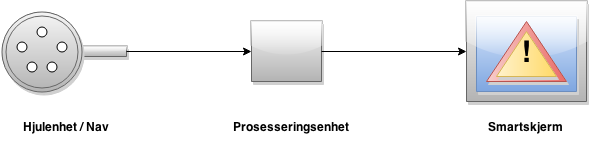
\includegraphics[width=1.00\textwidth]{images/arkitektur-overordnet.png}
	\label{fig:overordnet-ark}
	\caption{Overordnet arkitekturskisse.}
\end{figure}

Mer detaljert beskrivelse av arkitektur finnes i seksjon \ref{sec:arkitektur}


%TODO: Kontakte noen som kan gi informasjon om formatet til pakken i nivået over
%CAN nettverket. Det er ønskelig å vite hva som blir brukt i dagens bilssytemer.

\section{Hardware}

Løsningen for hardwaredesignet baserer seg på vibrasjonsmålinger, som diskutert
i forstudiet (ref). For å løse dette trengs vibrajsonsmålere, en forsterkere,
en mikrokontroller og en CAN controller. Mikrokontrolleren skal styre
samplingsvinduet til vibrasjons-/frekvensmålingene og pakke målingene i en serie
av frames som sendes over CAN nettverket. CAN kontrolleren kan legges til som en
egen komponent eller den kan være integrert i mikrokontrolleren. Forsterkerene er
nødvendig for å få justert nivået fra sensorene til et ønskelig nivå. Sensorene
kobles til ADC-enheten i mikrocontrolleren og oppløsnignen ADC'en
har innvirkning på hvilken båndbredde samplingen har. \\

Denne løsningen sentraliserer signalbehandlingen. Det vil si at hardware nøyer
seg med å sample signalet før det sendes til systemets sentrale
prosesseringsenhet. Da slipper man avansert hardware som DSP og man gjør det
lettere å oppdatere algoritmen som kjøres på signal-samplene.
